\documentclass[a4paper,twoside, 12pt]{report}

%% PACKAGES

\usepackage[english]{babel}
\usepackage{amsmath,amssymb,framed,graphicx,siunitx,enumerate,fancybox,marvosym,rotating}
\usepackage{marginnote,colortbl,lastpage,pgfplots,wasysym,ifthen,amsthm,datetime,lipsum}
\usepackage{tikz,circuitikz,hyperref,color,colortbl,float,cancel,multirow,arydshln}
\usepackage{wallpaper,changepage,fontawesome}

\usepackage[format=plain,font=it]{caption} % Caption italics om plaats te besparen

\usepackage[most]{tcolorbox}

\usepackage[a4paper,left=24mm,right=24mm,top=30mm,bottom=30mm]{geometry}
\usepackage{changepage}

\usepackage{tkz-fct}

\usepackage{pdfpages}
\usepackage{pdflscape}
\usepackage{titlesec, blindtext, color}
\usepackage{tabto}
\usepackage[font=small,labelfont=bf,tableposition=top]{caption}

\usetikzlibrary{calc,intersections,through,backgrounds,decorations.markings,decorations.pathmorphing}
\usetikzlibrary{arrows,automata,shapes,shapes.geometric,positioning,math,backgrounds,fadings}

\tikzset{
   ragged border/.style={ decoration={random steps, segment length=1mm, amplitude=1.2mm},
           decorate,
   }
}
\usepackage{pxfonts}

%% SETTINGS

\setlength{\parindent}{0cm}

\graphicspath{{pictures/}} 

\definecolor{azure}{rgb}{0.0, 0.5, 1.0}
\definecolor{mygreen}{rgb}{0.02, 0.5, 0.1}
\definecolor{goldenyellow}{rgb}{1.0, 0.87, 0.0}
\definecolor{bleudefrance}{rgb}{0.19, 0.55, 0.91}
\definecolor{gray75}{gray}{0.75}

\tcbset{colback=bleudefrance!10, colframe=bleudefrance}

\titleformat{\chapter}[hang]{\Huge\bfseries}{\thechapter\hsp\textcolor{gray75}{|}\hsp}{0pt}{\Huge\bfseries}
\titleformat{\section}
{\normalfont\Large\bfseries}{\thesection}{1em}{}
\titleformat{\subsection}
{\normalfont\large\bfseries}{\thesubsection}{1em}{}
\titleformat{\subsubsection}
{\normalfont\normalsize\bfseries}{\thesubsubsection}{1em}{}
\titleformat{\paragraph}[runin]
{\normalfont\normalsize\bfseries}{\theparagraph}{1em}{}
\titleformat{\subparagraph}[runin]
{\normalfont\normalsize\bfseries}{\thesubparagraph}{1em}{}

%% ENVIRONMENTS

\newtheoremstyle{break}
  {\topsep}{\topsep}%
  {\itshape}{}%
  {\bfseries}{}%
  {\newline}{}%
\theoremstyle{break}

\newtheorem{definition}{Definitie}
\newtheorem{theorem}{Stelling}
\newtheorem{corollary}{Gevolg}
\newtheorem{example}{Voorbeeld}
\renewcommand\qedsymbol{\textit{Qed}}

\newtheorem{remark}{Opmerking}

\newenvironment{solution}
  {
    \vskip 2mm
    \begin{adjustwidth}{11mm}{11mm}
        \textbf{Oplossing}:%
  }
  {  
    \end{adjustwidth}
    \vskip 4mm
  }

\newenvironment{mytcbox}[1]
  {
     \begin{equation}
       \begin{minipage}{#1}
         \begin{tcolorbox}   
           \begin{center} 
  } 
  {
           \end{center} 
         \end{tcolorbox}
       \end{minipage}
     \end{equation}
  }
\newcommand{\tempwidth}{50mm}

%% DEFINITIONS

\newcommand{\hsp}{\hspace{20pt}}

\newcommand\mystretch[1]{
  \begin{tikzpicture}
    \draw[white](0,0)--(0,#1);
  \end{tikzpicture}
}

\newcommand*\circled[1]{\tikz[baseline=(char.base)]{
            \node[shape=circle,draw,inner sep=2pt] (char) {\scalebox{0.6}{#1}};}}

\newcommand\MyTimeStamp[1]{
\begin{tcolorbox}[width=70mm,center]
\begin{center}
  \texttt{#1} \\ 
  \ \\ 
  \texttt{\today \ -\ \currenttime} \\
  \ \\
  \texttt{sander.speetjens@gmail.com} \\
\end{center}
\end{tcolorbox}
}

\newcommand\TotHier{
\begin{tcolorbox}[width=0.80\linewidth, colback=red!10, colframe=red, before skip=0mm, after skip=0mm]
\begin{center}
  \textbf{Tot hier nagekeken. (\today \ -\ \currenttime)}
\end{center}
\end{tcolorbox}
}

\newcommand\IN{\mathbb{N}}
\newcommand\ZZ{\mathbb{Z}}
\newcommand\IQ{\mathbb{Q}}
\newcommand\IR{\mathbb{R}}
\newcommand\IC{\mathbb{C}}

\newcommand\half{\hbox{$\frac{\small 1}{\small 2}$}}
\newcommand\Log[2]{{}^{#1}\!\log({#2})}
\newcommand\eff{e\!f\!\!f}
\newcommand\Reff{R_{\eff}}
\newcommand\keff{k_{\eff}}
\newcommand\Fext{F_{\!ext}}
\newcommand\Aext{A_{\!ext}}
\newcommand\omegaext{\omega_{\!ext}}
%\newcommand\euro[1]{\mbox{\hbox{\EUR}\ #1}}

\renewcommand{\parallel}{\mathbin{\!/\mkern-5mu/\!}}

\newcommand\MyGraphPre{}
\newcommand\MyGraphPost{}
\newcommand\EmptyGrid[5]{
  \begin{tikzpicture}[#5]
    \MyGraphPre
    \draw[step=1.0,gray,thin] (#1,#3) grid (#2,#4);
    \draw[thick,->] (#1-0.3,0)--(#2+0.3,0);
    \draw[thick,->] (0,#3-0.3)--(0,#4+0.3);
    \MyGraphPost
  \end{tikzpicture}
}

\newcommand{\LinkURL}[2][]
  {
     \ifthenelse{\equal{#1}{}}
       {
         \href{#2}{\texttt{#2}}
       }
       {
         \href{#2}{\texttt{#1}}
       }
  }

\newcommand\MyLissajous[4]{
  \begin{tikzpicture}[#4]
    \draw[->] (-1.2,0)--(1.2,0);
    \draw[->] (0,-1.2)--(0,1.2);    
    \draw[lissajouscolor, ultra thick] plot[smooth,domain=0:2*pi,samples=100] ({sin((#1*\x r))}, {sin((#2*\x r)+#3)});   
  \end{tikzpicture}
}

\newcommand\button[1]{
  \begin{tikzpicture}
    \node [draw=black,fill=blue!8,very thick,rectangle,rounded corners, 
           inner sep=1pt, inner ysep=4pt, minimum height=6mm] (box){
    \begin{minipage}{8mm}
        \begin{center}\texttt{#1}\end{center}
    \end{minipage}
    };
  \end{tikzpicture}
}

\newcommand\screen[1]{
  \framebox{  
    \begin{minipage}{30mm}
      {\ \hfill\texttt{#1}}
    \end{minipage}
  }
}

\newcommand\foton[6]{
  \tikzmath{
    real \rico, \cosa, \sina, \sll;
    \rico = (#2-#4)/(#1-#3); 
    \cosa = 1/(sqrt(1+\rico^2));
    \sina = \rico*\cosa; 
    \sll = 1; % lengte v.d. lijntjes voor en na de zigzag
  } 
  \draw[thick] (#1,#2)--(#1+\sll*\cosa,#2+\sll*\sina);
  \draw[thick, decoration = {zigzag,segment length = 2.5mm, amplitude = 1.5mm}, decorate] 
       (#1+\sll*\cosa,#2+\sll*\sina)--(#3-\sll*\cosa,#4-\sll*\sina);
  \draw[thick,->] (#3-\sll*\cosa,#4-\sll*\sina)--(#3,#4);
  \draw ({(#1+#3)/2},{(#2+#4)/2})node[#5]{#6};
}

\newcounter{TMPenumi}

%% HYPHENATION
\hyphenation{proef-on-der-vin-de-lijk}

\DeclareCaptionLabelFormat{andtable}{#1~#2  \&  \tablename~\thetable}

%% DOCUMENT

\begin{document}


%% FRONTMATTER

% Titlepage

\thispagestyle{empty}

\ \\
\begin{center}
  
\includegraphics[width=50mm]{ThomasMoreLogo.png}\\
  \vfill
  \dotfill \\
  \ \\
  \scalebox{2.9}{Smart Energy Meter (SEM)} \\
  \vskip 2.5mm
  \dotfill
  \vfill
  \scalebox{1.5}{Practice Enterprise}  \\
  \ \\
  \scalebox{1.2}{2021 - 2022}
  \vfill
  %\includegraphics[width=100mm]{FinishedProject.png}\\  
  \vfill
  \scalebox{1.0}{Sander Speetjens} \\
  
\includegraphics[width=10mm]{Logo.png} \\
  \scalebox{1.0}{1 Embedded Software} \\
\end{center}
\ \\

\eject

% Version Page

\thispagestyle{empty}

\begin{center}
  \ \\
  \vfill
  \MyTimeStamp{Version 1.0}
  \vfill

  \vfill\vfill
\end{center}

\eject

% Preface

\chapter*{Preface}
\thispagestyle{empty}
I'm Sander Speetjens, a first year student Electronics Embedded Software at Thomas More - Campus De Nayer.
\ \\ \ \\
This bundle will be a summary of all of the information that I gathered over the course of half a semester about my project Smart Energy Meter (SEM) or making my digital electricity meter more smart with a separate observation station. I had chosen this subject, because recently our energy supplier installed one of their new energy meters at home and I wanted to know our energy consumption. The system had to be reliable in the long term, but also consume little energy. This was quite challenging in terms of software, because there was a design constrained that we couldn't use any pre-written libraries or platforms like Arduino. With this practice enterprise, I want to demonstrate that I can apply my knowledge gained in secondary school and university to both the Electronic and Mathematical parts. Moreover, this was the perfect moment to focus on my favourite subjects, namely the combination of hardware, software and mathematics.
\ \\ \ \\
Because I could not have achieved all this without help from others, I would like to thank a few people. First and foremost, I would like to thank my teachers for assisting me with the technical and mathematical aspects of my practice entry.  I would also like to thank my friends who have worked together with me to make this possible.
Finally, I would also like to thank my parents, who have always supported me and helped me review my assignments.
\vfill
\eject

%empty page

\clearpage{\pagestyle{empty}\cleardoublepage}

% Table Of Contents

\setcounter{section}{0}
\setcounter{subsection}{0}

%\parskip=-0.41mm
\tableofcontents
\thispagestyle{empty}

\vfill

\eject

\vfill

\begin{figure}[H]
  \centering
  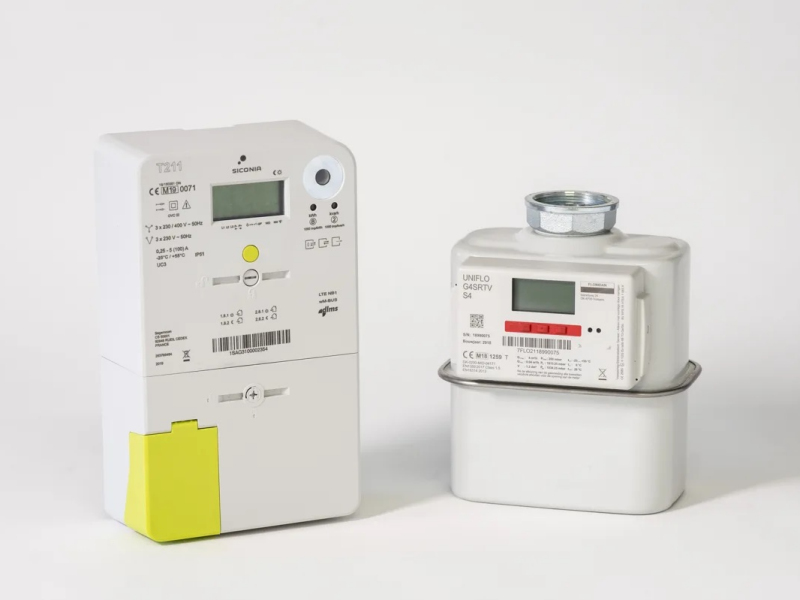
\includegraphics[width=0.9\textwidth]{SmartMeter.jpg}
  \caption{The new ''Smart Meter'' from Sagemcom}
\end{figure}

\eject


\chapter{Theory}

\section{The Smart Meter}

\subsection{Introduction}

The digital meters for electricity and gas were introduced in Flanders on 1 July 2019. Since then, they have replaced the old, mechanical meters that are no longer in circulation. Fluvius automatically installs them at new housing developments or renovations where the electricity connection is renewed. In addition, Fluvius launched a major geographical roll-out this spring to install such meters at every household and small business in Flanders. This will be organised by region, town or municipality. The roll-out aims at a complete conversion by 2029, with the main acceleration in the next three years. By the end of 2024, 80\% of homes should have digital meters.

\subsection{What is a Smart Meter}
A smart meter is an electronic device that records information such as consumption of electric energy, voltage levels, current, and power factor. Smart meters communicate the information to the consumer for greater clarity of consumption behavior, and electricity suppliers for system monitoring and customer billing. Smart meters typically record energy near real-time, and report regularly, short intervals throughout the day. Smart meters enable two-way communication between the meter and the central system. Such an advanced metering infrastructure (AMI) differs from automatic meter reading (AMR) in that it enables two-way communication between the meter and the supplier. Communications from the meter to the network may be wireless, or via fixed wired connections such as power line carrier (PLC). Wireless communication options in common use include cellular communications, Wi-Fi (readily available), wireless ad hoc networks over Wi-Fi, wireless mesh networks, low power long-range wireless (LoRa), Wize (high radio penetration rate, open, using the frequency 169 MHz) ZigBee (low power, low data rate wireless), and Wi-SUN (Smart Utility Networks).
\url{https://en.wikipedia.org/wiki/Smart_meter}

\eject

\subsection{Objective}
How to read the required data from the smart meter with my microcontroller. Wich protocol does it use and how do I translate the data to useable variables.

\subsection{Expectation}
I think that the meter will use a simple protocol like RS232 because it only uses 1 data signal and one ground for one-way comunication. I also expect that the meter will send out the data in clear text because it's easier to decipher then a custom data format.

\subsection{User-Ports}
These digital meters contain 2 User ports, which you are able to read you're consumption/production statistics from. The P1 port follows the DSMR 5 standard of the Dutch Smart Meter extended with the e-Mucs specification.
The S1 port provides a limited possibility of data and is going to be removed from the newer meters and is not going to be used in this project.

\subsection{Physical connection}

\begin{figure}[!ht]
  \centering
  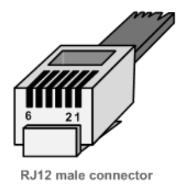
\includegraphics[width=3cm]{RJ12.png}
  \qquad
  \begin{tabular}{l|c} % <-- Alignments: 1st column left, 2nd middle with vertical lines in between
    \hline
    \textbf{Pin} & \textbf{Signal}   \\
    \hline
    1            & 5V power supply   \\
    2            & Data request (5V) \\
    3            & Data GND          \\
    4            & Not connected     \\
    5            & Data (open drain) \\
    6            & GND               \\
  \end{tabular}
  \captionlistentry[table]{RJ12 connector and the pinout for the P1 port}
  \captionsetup{labelformat=andtable}
  \caption{RJ12 connector and the pinout for the P1 port}
\end{figure}

\subsection{Internals of the meter}
\begin{figure}[H]
  \centering
  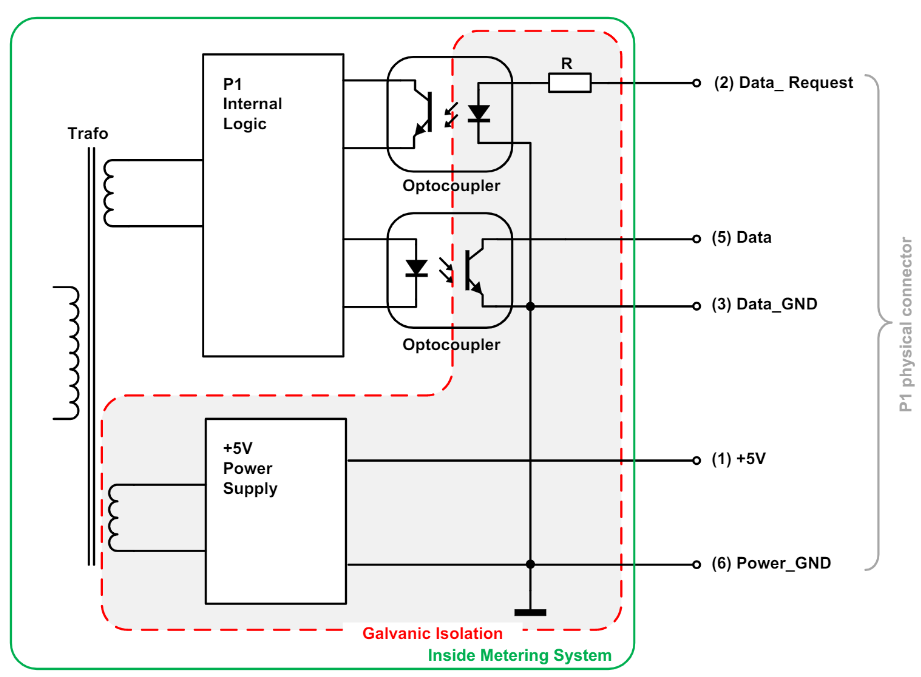
\includegraphics[width=0.9\textwidth]{MeterIntern.png}
  \caption{The internal workings of the Fluvius Meter}
\end{figure}
\subsubsection{+5V Power supply}
The P1 interface provides a stable +5V DC power supply via "+5V" (pin 1) and "GND"(pin 6) lines to provide a connected IoT device with a power source.

U = 5,0 V ( max = 5,5 V with I = 0 mA , min = 4,9 V with I = 250 mA )

\subsubsection{Data request}
The P1 port is activated (will start sending data) by setting "Data request" (pin 2) high (4,0V to 5,5V). While recieving data, this line must be kept high.

\textbf{Warning: To stop receiving data the "Data request" line must be put in a high impedance mode and must not be connected to the GND or 0V}

\subsubsection{Data}
Here we run into a problem, due to the use of optocouplers, the "Data" (pin 5) line must be designed as an Open Collector output and must be logically inverted or inverted via software before it can be used with IoT devices.

A "Data" line LOW has a voltage of 0,2 V (0 - 1V), HIGH has a voltage provided by a pull-up resistor to the VCC of the microcontroller with a maximum current of 30 mA.\ \\ \ \\

\subsubsection{Communication Protocol}
The interface must use a fixed transfer speed of 115200 baud. \ \\

The Fluvius Smart Meter sends its data to the connected IoT device every single second and the transmission of the entire P1 telegram is completed within 1s. \ \\

The format of transmitted data is defined as “8N1”. Namely:

\begin{itemize}
  \item 1 start bit,
  \item 8 data bits,
  \item no parity bit and
  \item 1 stop bit.
\end{itemize}

\subsubsection{Data readout}
The Fluvius Smart Meter transmits the data message, as described below, immediately following the activation through the Request signal.

\begin{figure}[!ht]
  \centering
  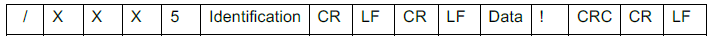
\includegraphics[width=10cm]{CommunicationExample.png}
  \qquad
  \caption{Photo of one transmission message}
\end{figure}

\subsubsection{End of transmission}
The data transmission is complete after the data message has been transmitted. An acknowledgement signal is not provided for.

\subsubsection{Data objects}

Go to the DSMR 5 standard and e-Mucs specification for more information.
\url{https://www.netbeheernederland.nl/_upload/Files/Slimme_meter_15_a727fce1f1.pdf}\\
and \url{https://www.fluvius.be/sites/fluvius/files/2019-12/e-mucs_h_ed_1_3.pdf}
\vfill
\eject

\section{Ethernet}
\subsection{Introduction}
Now we have our data,but we don't have a place to store it. The microcontroller doesn't have enough memory to store all of our data, so we have transfer this data to another system.
Here comes Ethernet/ WIFI to the rescue. Because it is used on every modern computer system it becomes super easy to implement, also our microcontroller is specially made to be an Internet of Things (IoT) device. Because it has a lot of features out of the box like WIFI, Ethernet and Bluetooth with it's prepackaged libraries or also known as stacks to make it super straight forward to use.

\subsection{What is ethernet}
This is a computer networking standard for Local Area and Wide Area Networks that is commonly used today.\\
See the link for more info:
\url{https://en.wikipedia.org/wiki/Ethernet}

\subsection{Objective}
How can we connect our microcontroller to another device over ethernet and with wich protocol are we going to use, that is both easy to use and widly used. In what format are we going to send our data over the air to that device.

\subsection{Expectations}
My background in computers says me that TCP/IP and HTTP are the most commonly used protocols over ethernet.

\subsection{TCP/IP and HTTP}
\subsubsection{What is TCP/IP}

The TCP/IP model was designed and developed by the US Department of Defense (DoD) in 1960s and is based on standard protocols. It stands for Transmission Control Protocol/Internet Protocol. The TCP/IP model is a concise version of the OSI model. It contains four layers, unlike seven layers in the OSI model.

\begin{enumerate}

  \item Network Access Layer

        This layer corresponds to the combination of Data Link Layer and Physical Layer of the OSI model. It looks out for hardware addressing and the protocols present in this layer allows for the physical transmission of data.
        ARP is a protocol of the Internet layer, but there is a conflict about declaring it as such or as a Network access layer protocol. It is described as residing in layer 3, being encapsulated by layer 2 protocols.


  \item Internet Layer

        This layer parallels the functions of OSI’s Network layer. It defines the protocols which are responsible for logical transmission of data over the entire network. The main protocols residing at this layer are :
        \begin{itemize}

          \item IP – stands for Internet Protocol and it is responsible for delivering packets from the source host to the destination host by looking at the IP addresses in the packet headers. IP has 2 versions:
                IPv4 and IPv6. IPv4 is the one that most of the websites are using currently. But IPv6 is growing as the number of IPv4 addresses are limited in number when compared to the number of users.
          \item ICMP – stands for Internet Control Message Protocol. It is encapsulated within IP datagrams and is responsible for providing hosts with information about network problems.
          \item ARP – stands for Address Resolution Protocol. Its job is to find the hardware address of a host from a known IP address. ARP has several types: Reverse ARP, Proxy ARP, Gratuitous ARP and Inverse ARP.
        \end{itemize}

  \item Host-to-Host Layer

        This layer is analogous to the transport layer of the OSI model. It is responsible for end-to-end communication and error-free delivery of data. It shields the upper-layer applications from the complexities of data. The two main protocols present in this layer are :
        \begin{itemize}

          \item Transmission Control Protocol (TCP) – It is known to provide reliable and error-free communication between end systems. It performs sequencing and segmentation of data. It also has acknowledgment feature and controls the flow of the data through flow control mechanism. It is a very effective protocol but has a lot of overhead due to such features. Increased overhead leads to increased cost.

          \item User Datagram Protocol (UDP) – On the other hand does not provide any such features. It is the go-to protocol if your application does not require reliable transport as it is very cost-effective. Unlike TCP, which is connection-oriented protocol, UDP is connectionless.
        \end{itemize}
\end{enumerate}
for more info go to\\
\url{https://www.geeksforgeeks.org/tcp-ip-model/}
\subsubsection{HTTP}
Hypertext Transfer Protocol (HTTP) is an application-layer protocol for transmitting hypermedia documents, such as HTML. It was designed for communication between web browsers and web servers, but it can also be used for other purposes. HTTP follows a classical client-server model, with a client opening a connection to make a request, then waiting until it receives a response. HTTP is a stateless protocol, meaning that the server does not keep any data (state) between two requests.
\paragraph{Methods}
HTTP defines a set of request methods to indicate the desired action to be performed for a given resource. Although they can also be nouns, these request methods are sometimes referred to as HTTP verbs. Each of them implements a different semantic, but some common features are shared by a group of them: e.g. a request method can be safe, idempotent, or cacheable. These are the most used once:

\begin{itemize}
  \item GET: The GET method requests a representation of the specified resource. Requests using GET should only retrieve data.
  \item POST: The POST method submits an entity to the specified resource, often causing a change in state or side effects on the server.
  \item PUT: The PUT method replaces all current representations of the target resource with the request payload.
  \item DELETE: The DELETE method deletes the specified resource.
\end{itemize}
for more info over http go to\\
\url{https://developer.mozilla.org/en-US/docs/Web/HTTP}

\subsection{Implementation}
We will use the HTTP and TCP/IP stack for handeling data. And we will use the HTTP Post method to send the data over the stack.

\vfill
\eject

\section{Containers, Webservers, Databases and Graphing}
\subsection{Introduction}
At this point we have the data send over the network and we need a way to receive it and store it in a safe place. Therefor we need to design the receiving and of the system on a PC, this handles the data storage side of the whole project.

\subsection{Objective}
\begin{itemize}
\item We have to handle the incomming HTTP Post request and put it in a database.
\item We have to choose which webserver we are going to use with which language.
\item We have to choose the database software.
\item We have to choose the graphing software.
\item We have to make it work a lot of PC's therefor it will have to be containerized via Docker.
\end{itemize}

\subsection{Software selection}
I'm going to use Free Open Source Software (FOSS) for this project.
For the database I will use MariaDB, for the webserver I'm using apache2 and I'm using PHP for server side scripting. For graphing I will use Grafana.

And for the containers I'm using Podman. This is a free and opensource alternative to Docker, developed by Red Hat.

\subsection{Realization}
For the realization I created a Pod, this is a way to combine multiple containers and let them talk to each other. We have to connect the ports that the pod uses to our system and give them permanent storage on our disk in the form of shared volumes.

Then we have to set up the database, create users with specific permissions and create the php script.

\chapter{Project specifications}
\section{Components used}
\begin{itemize}
  \item ESP32-WROOM\tabto{11cm}(€5)
  \item Raspberry Pi/ PC\tabto{11cm}(Free)
  \item Waveshare e-paper display 3.7 inch 480x280px\tabto{11cm}(€42,13)
  \item extra components\tabto{11cm}(€20)

\end{itemize}

\section{Proposed Project Specifications}
The project is composed out of 3 parts: The sensor, the database and an observation unit. \ \\
The sensor side of the project contains all of the hardware that converts the data from the digital energy meter and sends that data to the database over WIFI once every couple of minutes (1-5 min).
\ \\
The database stores all of the records in a table. The data is received and send via a web-interface written in PHP and can be received via http requests. There will also be a dashboard that can be accessed via a web browser. But this is not important for this project.
\ \\
The display is the most important part of this project because it is the only visible part and has to be eye catching. It contains a graphical e-paper display to display the graph, a rotary encoder to select the data format (day, week, month or year) and you are able to ask for a specific format as example date format "week, -2" that will be two weeks prior to now.
\ \\
All of the parts are powered by a 5V wall adapter.

\begin{landscape}
  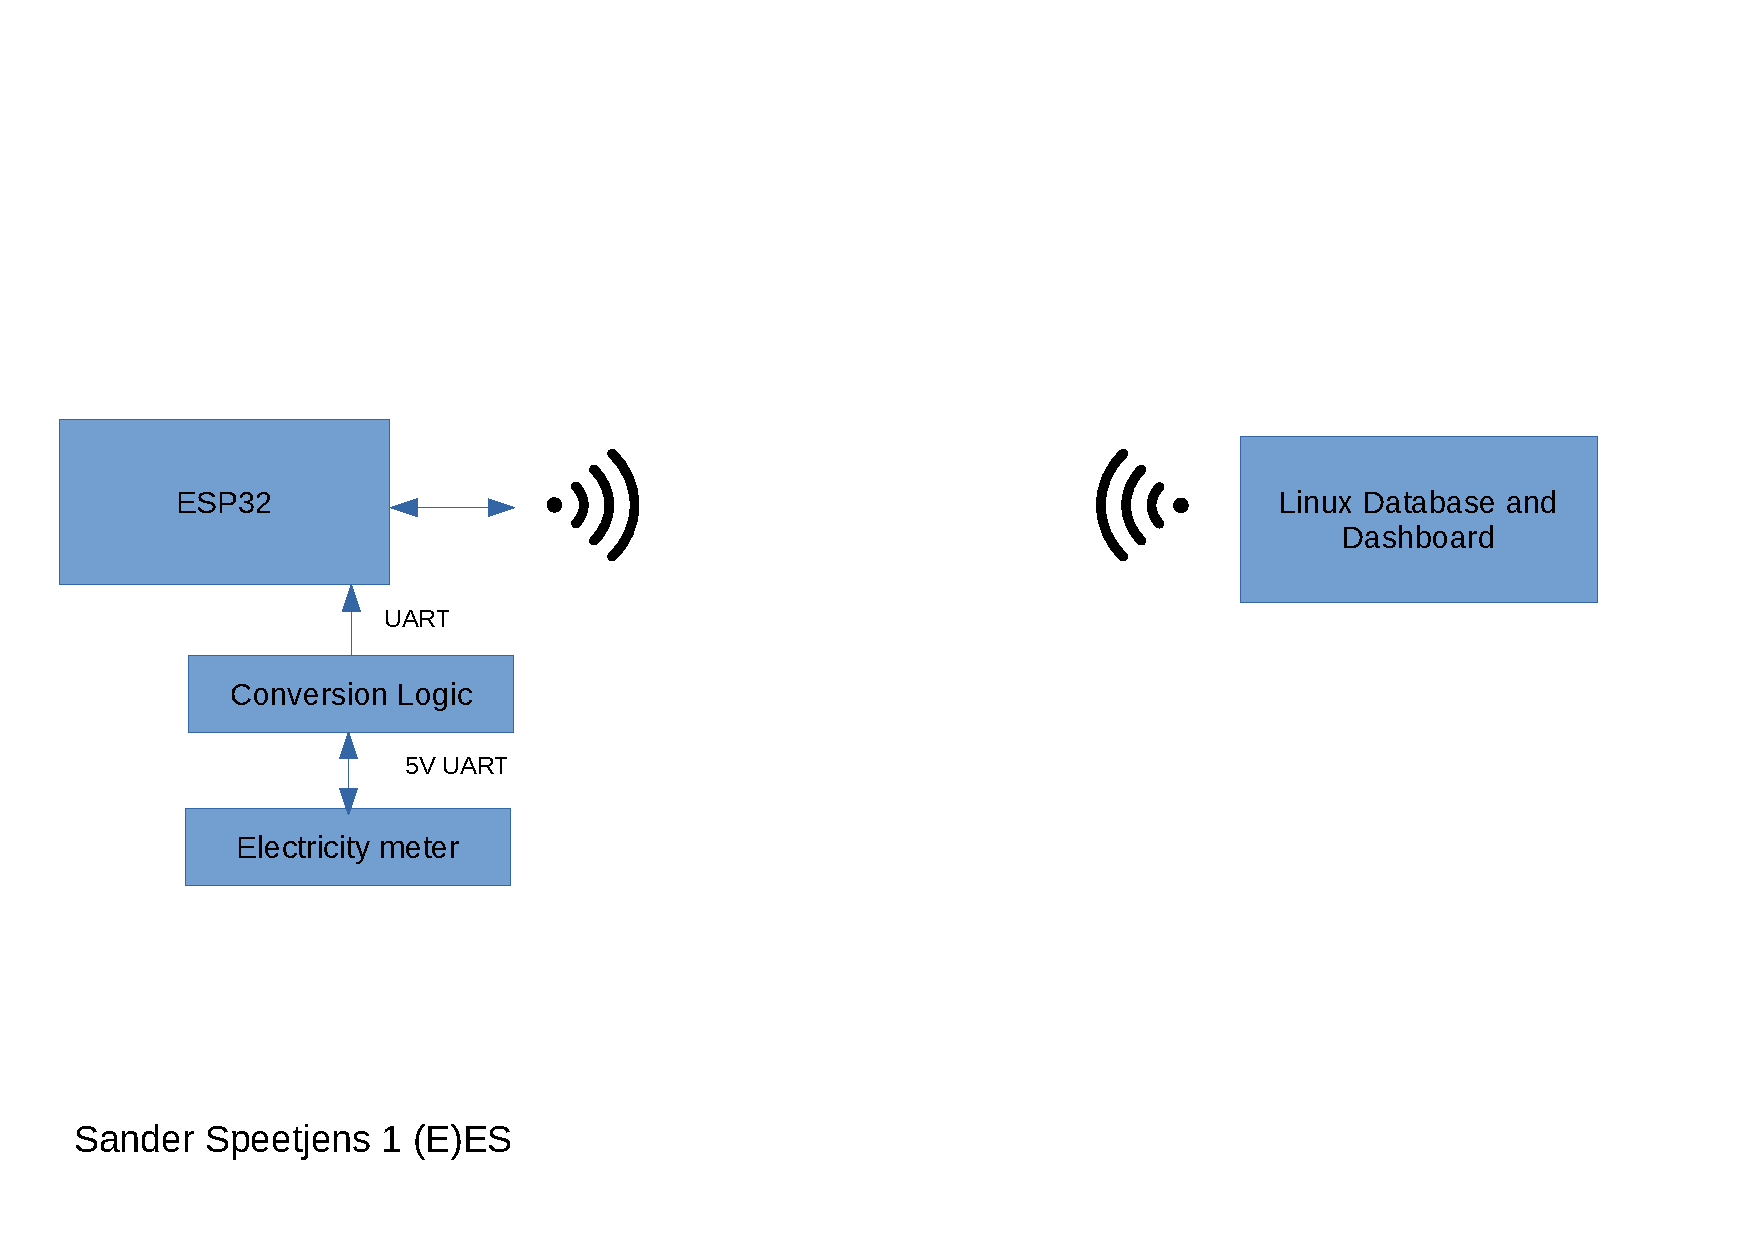
\includepdf[landscape=true, pagecommand=\section{Hardware Diagram}, pages=1]{Hardware.pdf}
\end{landscape}
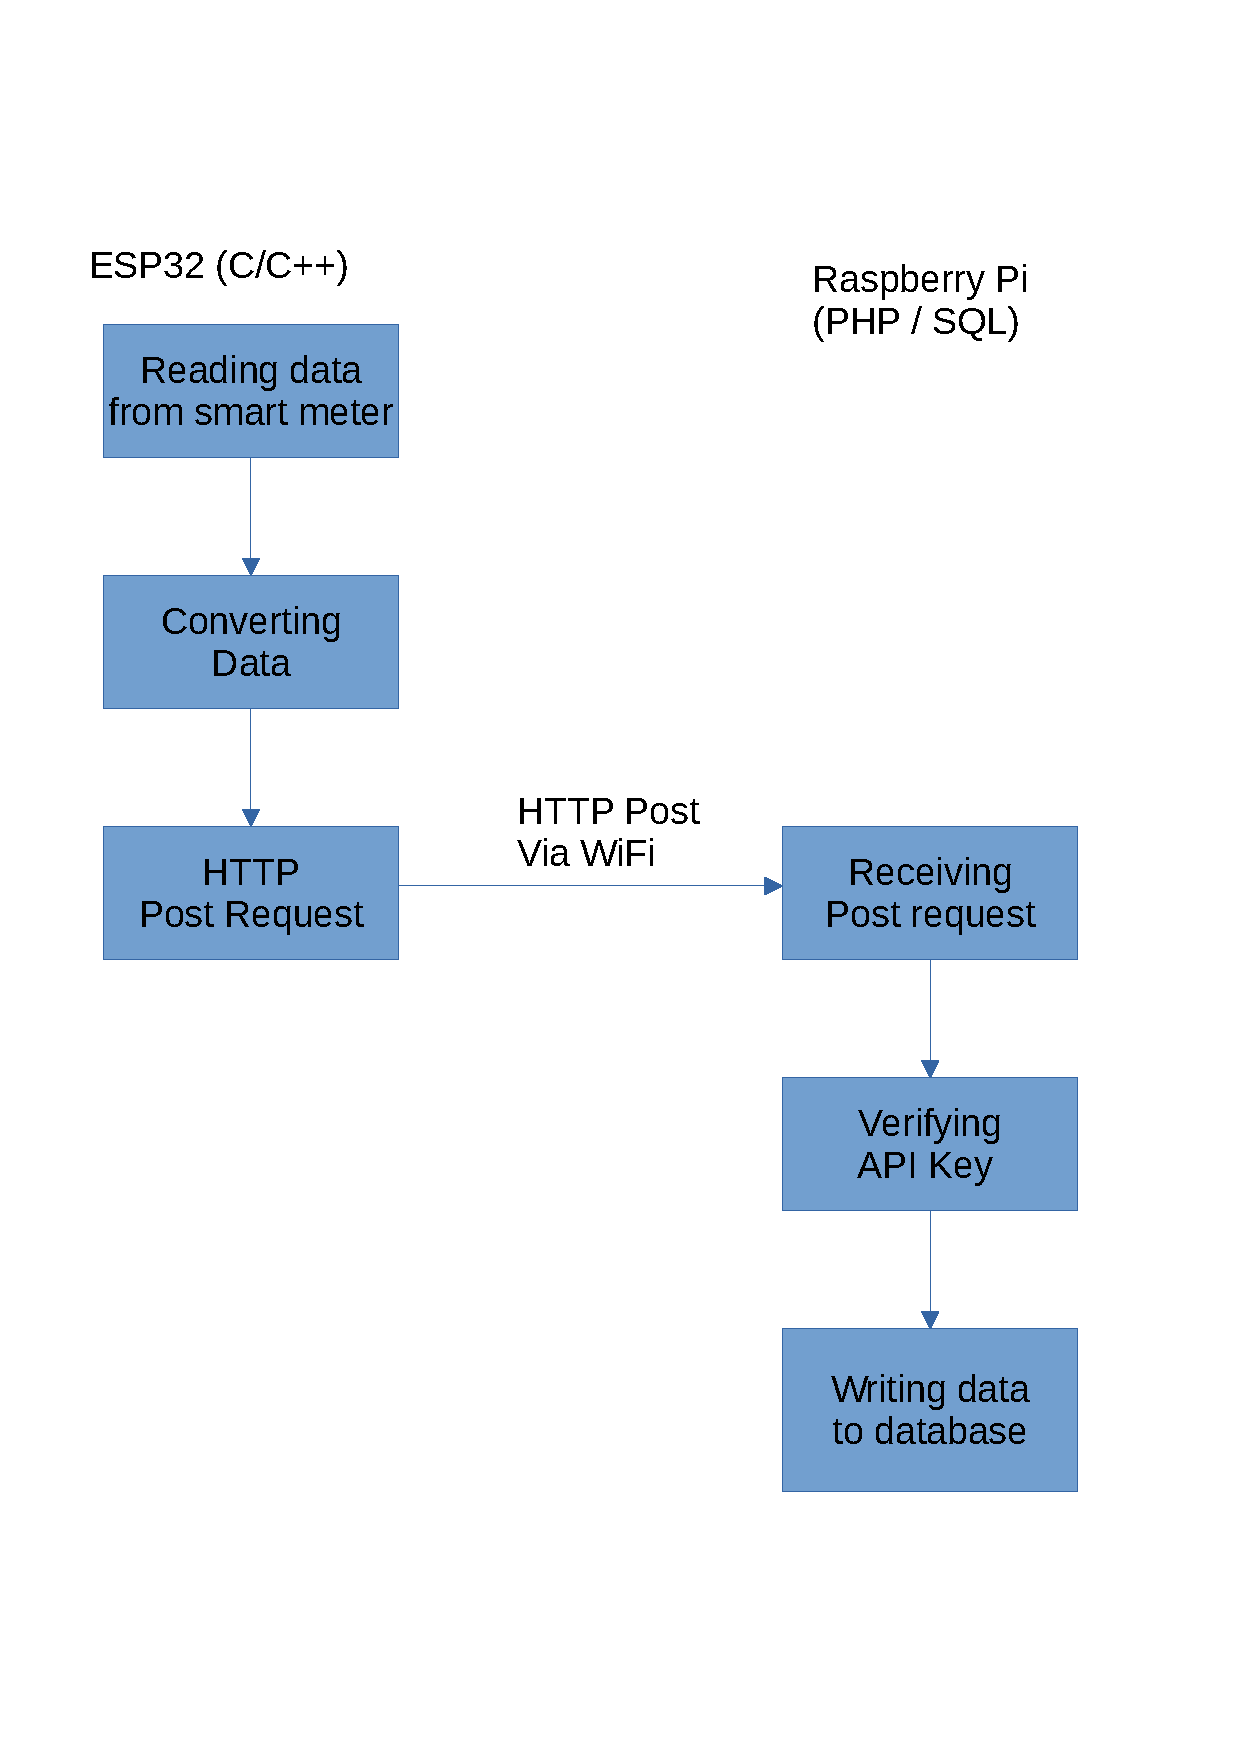
\includepdf[pagecommand=\section{Block diagram}, pages=-, scale=.95]{GIP-Blokschema-Programma.pdf}
\begin{landscape}
  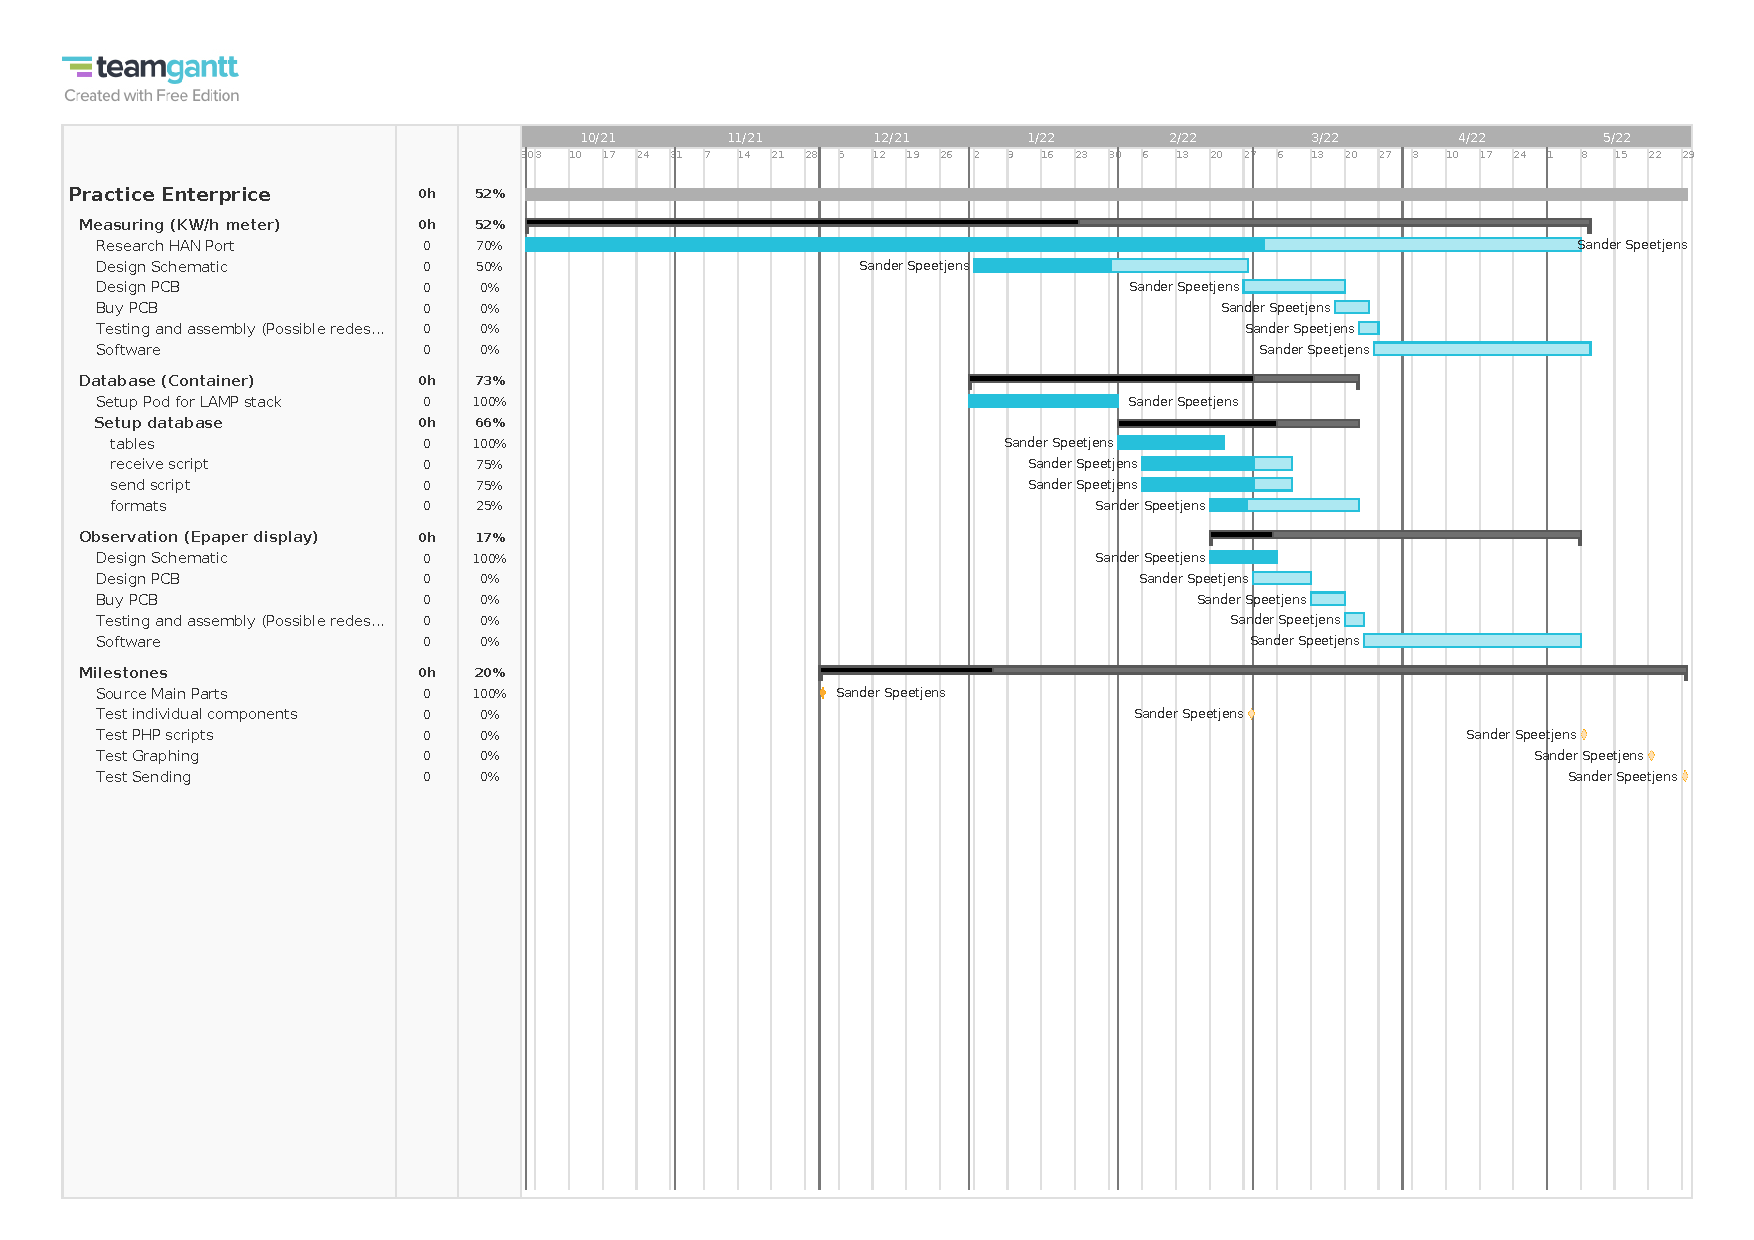
\includepdf[landscape=true, scale=.75, pagecommand=\section{Gantt Chart}, pages=1]{Gantt.pdf}
\end{landscape}

\chapter{The actual build}
\section{My Goals}
\begin{itemize}
\item Sensor\tabto{12cm}Reached\\
I'm able to read a mock message from a meter, decode it and send it to a database via an HTTP post request. The only part that didn't work was the PCB.
\item Database\tabto{12cm}Reached\\
I'm able to receive post and get requests and give or receive the required data back.
\item Display\tabto{12cm}Partly Reached\\
(only receiving and processing data) \\
Due to a lack of time, I only implemented the HTTP Get, data processing steps and high-level graphing functions.
\item Learn about the ESP32 and it's IDE\tabto{12cm}Reached\\
I'm able to initialize, build, upload and monitor projects via Microsoft Visual Studio Code. And I'm able to understand the documentation from Espressif.
\item Better understand how to use LaTEX for creating documents\tabto{12cm}Reached\\
This whole document is written in LaTEX with the exception of the blockdiagrams.
\end{itemize}
\vfill
\eject
\section{Details}
\begin{figure}[!ht]
  \centering
  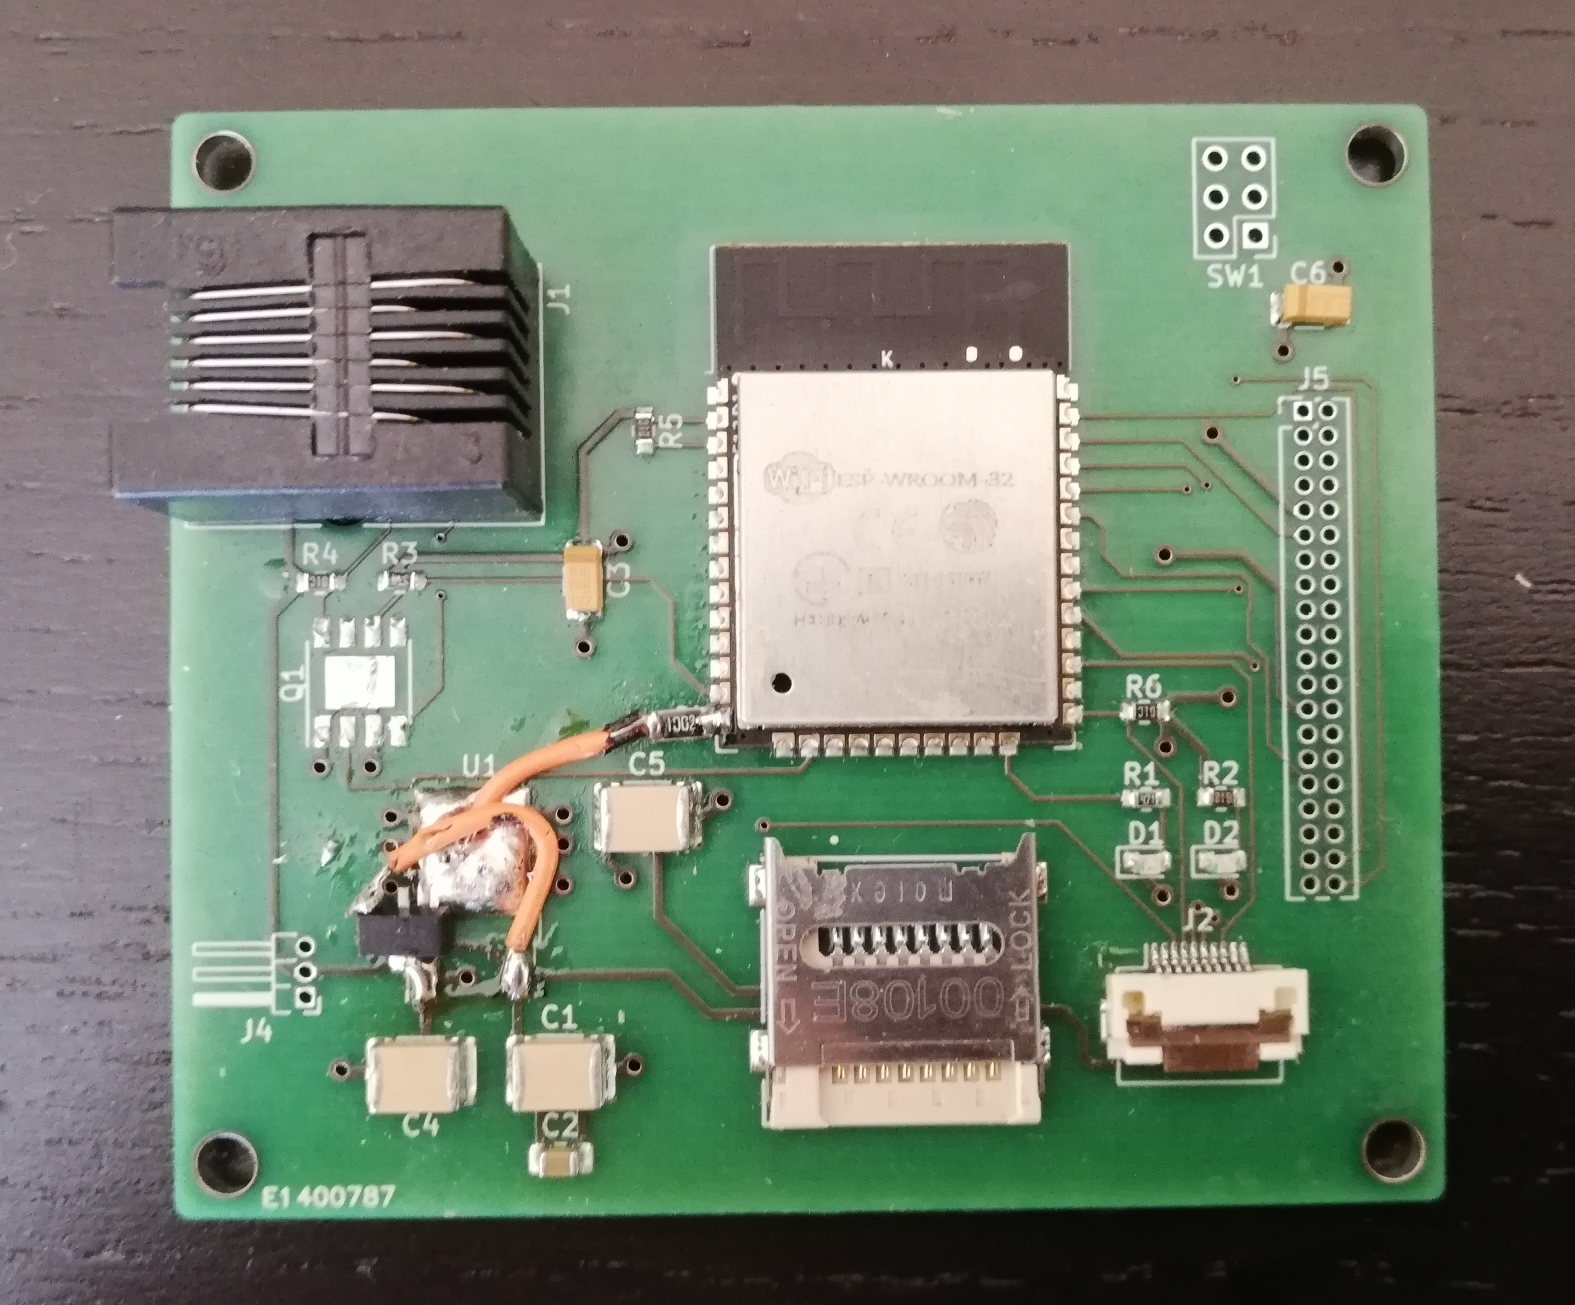
\includegraphics[width=6cm]{SEM.jpg}
  \qquad
  \caption{What my PCB looks like}
\end{figure}
\begin{itemize}
\item ESP32\\
The esp32 is a 32 bit dual core LX6 RISC V Microcontroller from Xtensa. Build for the purpose of IoT applications. It has 30 GPIO pins (6 are reserved for the SPI Flash), onboard UART, SPI, I2C and PWM. It also has 2-4MBytes of onboard flash.
\item Conversion Logic\\
The logic is pretty easy, the data pin is of type Open Drain, so we can just pull it up to 3V3 and we have an inverted UART signal that can be inverted via software. (uart\_set\_line\_inverse) For the enable line we need a tri-state buffer and a level shifter. (ESP (3V3) \textrightarrow Logic Shift (5V) \textrightarrow tri-stat buff (5V tri) \textrightarrow enable pin)
\item SD card\\
The SD-Card is connected to the VSPI pins, it has a FAT filesystem and contains one file config.txt which contains the necesary info to connect to wifi, the server ip, port, uri and API key. The code for the SD card is untested because I wasn't able to connect one to the ESP32.
In the format: configName=configText\textbackslash n
\item Display\\
I wanted to use a WaveShare Epaper dislay (3.7 inch, 4 colours), but I hadn't enough time to do anything with it. It is accesible via SPI with 2 extra control signals (command input or data and busy output)
\item Rotary Encoder\\
I wanted to use a rotary encoder with a switch to control select what data to show. I wanted to create a seporate task to check te rotary switch and report back to the main display task.
\item PCB \\
I gave up on my PCB after one month of troubleshooting , but I eventually figured out what the issue was. An overvoltage most likely destroyed both my ESP32 and my programmer.
And I only began writing code 2 weeks before the deadline because I was too focussed on trying to find the hardware mistake.
That's why I only finished the Sensor and Database side of the project. I ran out of time to write code and create documentation for my code.
\end{itemize}

\vfill

\section{Faults}
\begin{enumerate}
\item PCB\\
	I messed a lot up on my PCB, from ordering the right components to using the wrong footprint or even not buying the necessary components.\\
	\begin{itemize}
	\item I installed the wrong voltage regulators 5V and 1.2V which destroyed one of my ESP32's and my UART programmer.
	\item I bought the wrong type of Mosfets P-type instead of N-type
	\item I forgot that the Meter request pin is Tri-state and didn't add the buffer for it
	\item I switched around the RX and TX of the programming connector
	\item The footprint of the voltage regulator and the dislay connector where the wrong size
	\item I forgot to connect the Chip Select line of the Dislay
	\end{itemize}
	\item Software
	\begin{itemize}
		\item My stacksize in my readMeter task was too small and caused Exceptions
		\item I used a pin that was internally used for the SPI flash memory
		\item I put my uart\_set\_line\_inverse before I attached the driver ...
		\item I declared some variables as static in my "uart.c", but that caused my program to only work once
		\item I thought that I could give the uart\_read\_bytes function a pointer to one byte, but it expected an array because it uses the strings library (strncpy)
		\item I used some variables inside of statements and they weren't accesible anymore afther it moved out of the clause
		\item I forgot to include TLS libs, they where necessary for the http functions to work proparly, even if I didn't use HTTPS
	\end{itemize}
\end{enumerate}
\vfill
\eject
\section{Learning Curve}
There is a big difference between using a microcontroller like the XC888, ATMEGA32U4 (What I previously used) and the ESP32
\begin{itemize}
\item CPU architecture: intel 8051 assembly \verb|<=>| ATMEL RISC Core \verb|<=>|  Xtensa LX6 RISC V dual core processor
\item IO: Almost every IO function is available on evey pin ex every pin can be a UART pin or PWM etc
\item Task based instead of one flow with interrupts
\item The documentation is complicated, you have to know where to look for something
\item Almost impossible to program in Assembly because it has so much functionallity
\item On board WiFi, BL, BLE
\item TCP/IP stack via included libraries
\item ... (more them I'll ever need)
\end{itemize}
\section{Code}
For the code go to \url{http://www.github.com/Sani7/SEM/tree/main/Code} \ I'm not going to list my code in this document, there is just to much of it and it will become a mess. And you have a nice blockdiagram of it.
\section{Conclusion}
I'm happy whith what I'v learned so far. It could have been better, but everybody says that when looking back to a project. Although I was only able to finish 2 of the 3 parts, I still think I did a good job in the time I had.

\chapter{References}
\url{https://docs.espressif.com/projects/esp-idf/en/latest/esp32/api-reference/} was my best friend and guide.\\
And thanks to the people at netbeheernederland and Fluvius who made the specification available:\\
\url{https://www.netbeheernederland.nl/_upload/Files/Slimme_meter_15_a727fce1f1.pdf}\\
and\\ \url{https://www.fluvius.be/sites/fluvius/files/2019-12/e-mucs_h_ed_1_3.pdf}
\vfill
\eject
\end{document}